\underline{Nouveau cours du 16/11} \\

CCL du cours de la dernière fois 
\[
    R^\phi (\hat{h} ^{ \phi - \mathbb{E}R?}) - R^\phi (h ^\star , \phi )
.\]

\section{Relation between $ R^\phi  $ and $ R^{0/1} $  }
In this section, no empirical proof, no n
\begin{itemize}
    \item $ R^\phi(h) = \mathbb{E}[\phi (- Y h(X))]  $ 
    \item $ R^{0/1}(h) = \mathbb{E}[ \mathbbm{1}_{Y \neq sign(h(X))} ] $ 
    \item $ \phi  $ = hinge / logistic / least square
\end{itemize}

\begin{lem}[]
    If $ \phi  $ is diff, convex, increasing, then $ sign(h^{\star, \phi }) = f^{\star, Bayes} $ with $ h^{\star, \phi }  \in  \arg \min_h R^\phi (h)$ 
\end{lem}
\begin{proof}[Proof:]
    \begin{enumerate}
        \item \begin{align*}
            R^\phi (h) &= \mathbb{E}[\phi (-Yh(X))(\mathbbm{1}_{Y=1} + \mathbbm{1}_{Y = -1}) | X] \\ 
                &= \mathbb{E}[\phi (-h(X)) \eta (X) + \phi (h(X)) (1 - \eta (X))]
        \end{align*}
        with $ \eta (X) = P(Y=1 | X) $
        
        \item Define $ H_\phi (p, \eta ) := \eta \phi (-p) + (1 - \eta ) \phi (p) $ and $ p^{\star , \phi }(\eta ) = \arg \min H_\phi (p, \eta ) $ (assuming existence for now) \\
        $ h^{\star , \phi }  $ minimizes $ R^\phi  $  and is such that for any fixed $ x $ 
        \[
            h^{\star , \phi }(x) = p^{\star , \phi }(\eta (x))
        .\]
        $ \forall h, R^\phi (h) - R^\phi (h^{\star , \phi }) = \mathbb{E}[H_\phi (h(X), \eta (X)) - H_\phi (h^{\star , \phi }(X), \eta (X))] $ 
        
        \item Example for Least Square : \begin{align*}
            H_\phi (p, \eta ) &= \eta (1 - p)^2 + (1 - p)(1 + p)^2 \\
            \frac{\partial H_\phi }{\partial p} (p , \eta ) &= 2 (p -1) \eta + 2(1 - \eta )(1+p) \\
                    &= 0 \Leftrightarrow p = 2 \eta - 1
        \end{align*} 


        See Table \ref*{table:loss}
        
        In all cases, $ sign(p^{\star , \phi }(\eta (X)) = sign(\eta (X) - 1/2)) = sign(h^{\star , \phi }(X)) = f^{\star , Bayes}$ 

        \item In general with $ \phi  $ strictly increasing, diff, convex, when $ \phi (t) \to _{t \to +\infty } + \infty $  $ \forall \eta \in ]0, 1[, H_\phi (\eta , p) \to _{p \to  \pm \infty } + \infty $ . Thus $ p^{\star , \phi }(\eta ) $ exists. And $ p \mapsto H_\phi (p, \eta ) $ is diff 
        \[
            \frac{\partial H_{\phi }}{\partial p} (p , \eta ) = 0 \Leftrightarrow \eta \phi ' (-p^{\star , \phi }(\eta )) = (1 - \eta ) \phi (p^{\star , \phi } (\eta )) 
        .\]
        \begin{enumerate}
            \item If $ \eta < 1/2 $, then $ \eta < 1 - \eta \Rightarrow  \phi ' ( p^{\star , \phi } (\eta )) > \phi ' (p^{\star , \phi } (\eta )) \Rightarrow  p^{\star , \phi } ( \eta ) \leq 0$ 
            \item If $ \eta > 1/2 $ ... $ \Rightarrow p^{\star , \phi } \geq 0 $ 
        \end{enumerate}
    \end{enumerate}
    Finally, $ sign(p^{\star , \phi } ( \eta ) = sign( \eta - 1/2) ) $ and thus $ sign(h^{\star , \phi } (X) ) = f^{\star , Bayes } (X)$  

\end{proof}

\begin{table}[!ht]
    \centering
    \begin{tabular}{|l|l|l|}
    \hline
        Loss & $ p^{\star , \phi }(\eta ) $  & $ \min H_\phi (p, \eta ) $  \\ \hline
        LS : $ (1 + v)^2 $  & $ 2 \eta - 1 $  & $ 4 \eta (1 - \eta )  $  \\ \hline
        Hinge & sign & a \\ \hline
        Logistic & a & a \\ \hline
    \end{tabular}
    \label{table:loss}
\end{table}


\begin{lem}[Zhang]
    Assume $ phi $ increasing, convex such that $ \phi (0) = 1 $. For $ \gamma \geq 1 $ we have $ \left| \eta  - 1/2 \right|^\gamma  \geq c \left| 1 - H_\phi (p^{\star , \phi }(\eta ), \eta ) \right|   $ . \\
    $ \forall h $ classifier $ h: \mathcal{X} \to \mathbb{R} $ 
    \[
        R^{0/1} (sign(h)) - R^{0/1}(f^{\star , Bayes}) \leq 2 c ^{1/\gamma }(R^\phi (h) - R^\phi (h^{\star , \phi }))
    .\]
\end{lem}

When $ h $ approximately minimizes the relaxed excess risk its $ sign(h) $ behaves well in terms of the initial excess risk !!. 

\begin{note}[]
    Note that $ \gamma = 2 $  for the square loss and the logistic loss. And that $ \gamma = 1 $ for the hinge loss. \\
    (we do not care about $ c $ )
\end{note}

\begin{proof}[Proof:]
    \begin{align*}
        R^{0/1} (sign(h)) - R^{0/1}(f^{\star , Bayes }) &= \mathbb{E}[ \mathbbm{1}_{sign(h(X)) \neq  f^{\star , Bayes}(X) 2  \left| \eta (X) - 1/2 \right| }] \\
        \text{(jensen, (1) )} &\leq \mathbb{E}[ \mathbbm{1}_{sign(h(X)) \neq  f^{\star , Bayes}(X) 2^\gamma  \left| \eta (X) - 1/2 \right| ^\gamma }]^{1/\gamma } \\
                        &\leq 2 c^{1/\gamma } \mathbb{E}[\mathbbm{1}_{sign(h(X)) \neq  f^{\star , Bayes}(X) } (1 - H_ \phi (p^\star _\phi  (\eta (X)) , \eta (X))]^{1/\gamma} (\eta (X) = P (Y=1 | X))
    \end{align*}
    \begin{note}[]
        Note that when $ sign(h(X)) \neq sign(\eta (X) - 1/2) $, then $ H_\phi ^\prime ( h(X), \eta (X) ) > 1 $. Indeed, $ \eta \phi (-p) + (1 - \eta ) \phi (p) \geq \phi ( - \eta  p + (1 - \eta ) p) = \phi ((1 - 2 \eta ) p )$ because $ \phi  $ convex. And now $ \phi ((1 - 2 \eta ) p) \geq  \phi (0) = 1 $ because $ \phi  $ increasing $ \geq 0 $ when $ sign(p) \neq sign(\eta - 1/2) $ 
    \end{note}
    
    \begin{align*}
        (1) &\leq  2 c^{1/\gamma } ( \mathbb{E} [ H( h(X), \eta (X)) - H(p^{\star , \phi }(\eta (X)), \eta (X)) ])^{1/\gamma } \\ 
            &= 2c ^{1/\gamma } ( R^\phi (h) - R^\phi (h^{\star , \phi }) )^{1/\gamma }
    \end{align*}
    
\end{proof}

CCL : $ \forall \hat{h} $ 
\begin{align*}
    R^{0/1} ( sign(\hat{h}) ) - R^{0/1} (f^{\star , Bayes }) \leq c^{1/\gamma } ( R^\phi (\hat{h}) - R^\phi (h^{\star , \phi }))^{1/\gamma } \\
    R^\phi ( \hat{h} ) - R^\phi ( h^{\star , \phi } ) = R^\phi (\hat{h}) - R^\phi (h^{\star , \phi }_\mathcal{F} ) + R^\phi (h^{\star , \phi }_\mathcal{F}) - R^\phi ( h^{\star , \phi } ) 
\end{align*}
where \begin{itemize}
    \item $ h^{\star , \phi }_\mathcal{F} \in \arg \min R^\phi (h) $ 
    \item $ R^\phi (h^{\star , \phi }_\mathcal{F}) - R^\phi ( h^{\star , \phi } ) $  approx error
\end{itemize}



\begin{align*}
    R^phi (\hat{h}) - R^\phi (h^{\star , \phi }_\mathcal{F}) &= R^\phi (\hat{h}) - \hat{R}^\phi_n(\hat{h}) (\leq  \sup _\mathcal{F} \hat{R}_n - R^\phi ) \\
        &+ \hat{R}^\phi _n (\hat{h}) - \hat{R}^\phi _n (\hat{h}^{\phi ERM}) \text{("optim error")} \\
        &+ \hat{R}^\phi _n (\hat{h}^{\phi-ERM}) - \hat{R}^\phi _n (\hat{h}^{\star , \phi } _\mathcal{F}) (\leq 0) \\
        &+ \hat{R}^\phi _n (h^{\star , \phi } _\mathcal{F}) - R^\phi (h^{\star , \phi } _ \mathcal{F}) (\leq \sup _\mathcal{F} \hat{R}^\phi _n - R^\phi )
\end{align*}
\textbf{Since the estimation error typically scales in $ O(\frac{1}{\sqrt[]{n}}) $ , no need to reach the ERM using our optimization algo !!.}

\begin{note}[]
    When using Lipschitz fonctions, we obtain slow rates $ O(\frac{1}{\sqrt[]{n}}) $. Is there a path towards fast rates ? Let's take the example of the mean estimation. 
    \begin{enumerate}
        \item Method 1 : \begin{align*}
            \hat{\theta } &= \frac{1}{n} \sum_{i=1}^{n} Z_i = \arg \min_\theta \frac{1}{2n} \sum_{i=1}^{n} (Z_i - \theta )^2  \\
            \theta ^\star &= \arg \min \frac{1}{2}\mathbb{E}[ (\theta - Z) ^2] = \mathbb{E}[Z]
        \end{align*}
        From the developpement before on the estimation error 
        \[
            R(\hat{\theta }) - R(\theta ^\star ) = O( \frac{1}{\sqrt[]{n}})
        .\]
        
        \item Method 2 : Direct computation \begin{align*}
            &R (\theta ) = \frac{1}{2}\mathbb{E}[(\theta  - Z)^2] = \frac{1}{2}(\theta - \mathbb{E}[Z])^2 + \frac{1}{2}Var(Z) \\
            &\Rightarrow R(\hat{\theta }) - R(\theta ^\star ) = R(\hat{\theta }) ( R(\mathbb{E}[Z])) = \frac{1}{2}(\hat{\theta } - \mathbb{E} (Z))^2 (\text{conditionallty to } \mathcal{D}_n)\\
            &\mathbb{E}_{D_n} [     ] = \frac{1}{2} \mathbb{E}[(\frac{1}{n} \sum_{}^{} Z_i - \mathbb{E}[Z])^2 ] = \frac{1}{2 \mathbf{n}} Var(Z) ( \mathbf{n} \text{ is FAST RATE } O(\frac{1}{n}))
        \end{align*}
        Bound only for this specific $ \hat{\theta } $ and because I also have stong convexity. 
        
        In supervised learning, fast rates can be established for strongly convex function (in our relaxed risks)
    \end{enumerate}
\end{note}

\chapter{Basics of deterministic optimisation}

In ML, construct a predictor often boils down to minimize an empirical risk using iterative algorithms.

\section{First order method}

\subsection{Basics of convex analysis}
$ F: \mathbb{R}^d \to \mathbb{R} $ convex, diff, L-smooth (its gradient is L-Lipschitz). 
\begin{itemize}
    \item convexity (under chords) : $ F(\eta \theta + (1 - \eta ) \theta ^\prime ) \leq  \eta F(\theta ) + (1 - \eta ) F(\theta ^\prime ), \forall \theta , \theta ^\prime , \forall \eta  \in 
    [0, 1] $ 
    \item If we add diff (tangent lie below) we have $ F(\theta ^\prime ) \geq F(\theta ) + \langle  \nabla F(\theta ) , \theta ^\prime - \theta  \rangle ,  \forall \theta , \theta ^\prime $ 
    \item (increasing slopes) $ \langle \nabla F(\theta ) - \nabla F(\theta ^\prime ), \theta - \theta ^\prime \rangle \geq 0 $ ($ \nabla F $ is said to be a monotone operator )
    \item if we add $ \mathcal{C}^2 $ (curves upwards) $ \forall \theta , Hess_F (\theta ) \succeq 0 $ (SDP)
\end{itemize}

$ \mu \text{-strongly}$ convex, $ \mu > 0 $. 
\begin{itemize}
    \item convexity (\textbf{"well"} under chords) : $ F(\eta \theta + (1 - \eta ) \theta ^\prime ) \leq  \eta F(\theta ) + (1 - \eta ) F(\theta ^\prime ) - \frac{\eta (1 - \eta ) \mu }{2} \left\| \theta - \theta ^\prime  \right\| ^2 _2 , \forall \theta , \theta ^\prime , \forall \eta  \in 
    [0, 1] $ 
    \item If we add diff (tangent lie \textbf{"well"} below) we have $ F(\theta ^\prime ) \geq F(\theta ) + < \nabla F(\theta ) , \theta ^\prime - \theta  > + \frac{\mu }{2} \left\| \theta - \theta ^\prime  \right\|^2_2, \forall \theta , \theta ^\prime  $ 
    \item (\textbf{"well"}increasing slopes) $ \langle \nabla F(\theta ) - \nabla F(\theta ^\prime ), \theta - \theta ^\prime \rangle \geq 0 + \mu \left\| \theta - \theta ^\prime  \right\| _2 ^2  $
    \item if we add $ \mathcal{C}^2 $ (curves upwards) $ \forall \theta , Hess_F (\theta ) \succeq \mu Id $ (SDP)
\end{itemize}
Other definition:
\begin{itemize}
    \item $ F $ is $ \mu \text{-strongly} $ convex $ \forall \theta _0, \theta \mapsto F(\theta ) - \frac{\mu }{2} \left\| \theta  - \theta _0 \right\|^2 _2 $ is convex.
    \item L-Smooth : $ \forall \theta , \theta ^\prime, \left\| \nabla F(\theta ) - \nabla F(\theta ^\prime ) \right\| \leq  L \left\| \theta - \theta ^\prime  \right\| $ 
\end{itemize}

\begin{lem}[Descent lemma]
    Assume that $ F $  is L-Smooth. Therefore $ \forall \theta , \theta ^\prime \in  $ domain of $ F $ 
    \[
        F(\theta ^\prime ) \leq  F(\theta ) + \langle \nabla F(\theta ) , \theta ^\prime  - \theta \rangle + \frac{L}{2} \left\| \theta ^\prime  - \theta  \right\| 
    .\]
\end{lem}
\begin{proof}[Proof:]
    \begin{align*}
        F (\theta ^\prime ) 
            &= F(\theta ) + \int_{0}^{1} < \nabla F(\theta  + t(\theta ^\prime - \theta )), \theta ^\prime - \theta > dt \\
            &= F(\theta ) \mathbf{+} < \nabla F(\theta ), \theta ^\prime  - \theta > + \int_{0}^{1} < \nabla F(\theta  + t(\theta ^\prime - \theta )) \mathbf{-} \nabla F(\theta ), \theta ^\prime  - \theta > dt \\
            &\leq F(\theta ) \mathbf{+} \langle \nabla F(\theta ), \theta ^\prime  - \theta \rangle + \int_{0}^{1} \left\| \nabla F(\theta + t(\theta ^\prime  - \theta )) - \nabla F(\theta ) \right\| \left\| \theta  ^\prime - \theta  \right\| dt \\
            &\leq F(\theta ) \mathbf{+} \langle \nabla F(\theta ), \theta ^\prime  - \theta \rangle + \int_{0}^{1} t L \left\| \theta ^\prime  - \theta  \right\|^2 dt \\
            &\leq F(\theta ) \mathbf{+} \langle \nabla F(\theta ), \theta ^\prime  - \theta \rangle + \frac{1}{2} L \left\| \theta  ^\prime  - \theta  \right\| ^2 _2
    \end{align*}
\end{proof}

\paragraph*{Consequence of this quadratics upper bound }

\begin{enumerate}
    \item \begin{align*}
        F(\theta ) &\leq F(\theta ^\star ) + \langle \nabla F(\theta ^\star ) , \theta  - \theta ^\star \rangle + \frac{L}{2} \left\| \theta - \theta ^\star  \right\| ^2 \\
        F(\theta ) - F(\theta ^\star ) &\leq \frac{L}{2} \left\| \theta  - \theta ^\star  \right\| ^2 
    \end{align*}
    \item 
    \[
        \min_\theta  F(\theta ) \leq \min _\theta F(\theta ) + \langle \nabla F(\theta ), \theta ^\prime - \theta \rangle  + \frac{L}{2}\left\| \theta ^\prime - \theta  \right\| ^2
    .\]
    $ \min _\theta F(\theta ) + \langle \nabla F(\theta ), \theta ^\prime - \theta \rangle  + \frac{L}{2}\left\| \theta ^\prime - \theta  \right\| ^2 $  is reach for $ \theta ^\prime  = \theta - \frac{1}{L} \nabla F(\theta ) $ 
    \begin{align*}
        &\leq F(\theta ) + \langle \nabla F(\theta ), \theta  - \frac{1}{L} \nabla F(\theta ) - \theta  \rangle + \frac{L}{2} \left\| \theta  - \frac{1}{L} \nabla F(\theta ) - \theta  \right\| ^2 \\
        &= F(\theta ) - \frac{1}{2L} \left\| \nabla F(\theta ) \right\| ^2
    \end{align*}

    All in all, $ \forall \theta  $ 
    \[
        \frac{1}{2L} \left\| \nabla F(\theta ) \right\| ^2 \leq  F(\theta ) - F(\theta ^\star ) \leq  \frac{L}{2} \left\| \theta  - \theta ^\star  \right\| ^2
    .\]
\end{enumerate}

\begin{note}[]
    In what follows, we could easily extend the study to non-diff function by involving \textbf{subgradients}. 
    
    $ F: \mathbb{R}^D \mapsto \mathbb{R} $ A vector $ \eta  \in \mathbb{R}^d $ is a subgradient of $ F $ at $ \theta  $ if 
    \[
        \forall \theta ^\prime, F(\theta ^\prime ) \geq F(\theta ) + \langle \eta , \theta ^\prime - \theta \rangle
    .\]
    $ \partial F(\theta ) $ is the subdifferential of $ F $ at $ \theta  $ a,d gathers all the subgradients of $ F $ at $ 0 $ i.e. the direction of hyperplanes passing through $ (\theta , F(\theta )) $ but remaining below the graph of $ F $ 

    \begin{figure}[h]
        \centering
        \includegraphics*[width=.5\textwidth]{figs/subgradients.jpg}
        \caption{subgradients}
    \end{figure}

\end{note}


\subsection{Gradient algorithms}
$ \theta ^\star = \arg \min F $ assuming existence and uniqueness. 

\subsubsection{Gradient algo}
\begin{enumerate}
    \item Init $ \theta _0  \in \mathbb{R} ^d $
    \item $ \forall t \geq 0, \theta _{t+1} = \theta _t - \gamma _{t+1} \nabla F(\theta _t) $ with $ \gamma _{t+1} $ gradient steps / learning rates
\end{enumerate}
Choice of steps : 
\begin{itemize}
    \item Constant step sizes $ \gamma _t = \gamma , \forall t $ it may depend on the time horizons $ T: \forall t \in [0, 1], \gamma _t = \gamma (T) $ 
    \item Line search : optimal step size at each iteration. $ \gamma _{t} = \arg \min _{\gamma > 0} F(\theta _{t-1} - \gamma \nabla F(\theta _{t-1}))) $. You can forget about that case in online algo!
\end{itemize}

\subsubsection{Link with the gradient flow}
The iterates of Gradient Descent (GD, Euler, XVIIIe)
\[
    \theta _{t+1} = \theta _t - \gamma _t \nabla F(\theta _t)
.\]
can be rewrittent as 
\[
    \frac{\theta _{t+1} - \theta _t}{\gamma _t} = - \nabla F(\theta _t)
.\]
Make the step size $ \gamma _t $ shrink to $ 0 $, we obtain the ODE 
\[
    \frac{\partial \theta }{\partial t} (t) = - \nabla F(\theta (t))
.\]
This continuous version is called the Gradient Flow (GF). Thus GD is a discretization of GF (using finite differences).

$ \nabla F(\theta ) $ is orthogonal to $ \{\theta ^\prime : F(\theta ^\prime ) = F(\theta )\} $ (level set) so that $ \frac{\partial \theta }{\partial t} (t) = \theta (t) $ point inwards $ \{\theta ^\prime : F(\theta ^\prime ) \leq F(\theta ) \} $ which guarantees that $ F(\theta (t)) $ is decreasing. \\
Indeed $ \frac{\partial (F \circ \theta )}{\partial t}(t) = \langle \nabla F(\theta (t)), \dot{\theta }(t) \rangle = - \left\| \nabla F(\theta (t)) \right\| ^2  $ 

\begin{thm}[]
    For $ F $ an L-Smooth. for $ \gamma _t = \gamma , \forall t $ with $ \gamma < 2/L $ 
    \[
        F(\theta _t) - F(\theta ^\star ) \leq \frac{\left\| \theta _0 - \theta 
        ^\star  \right\| }{2 \gamma (1 - \frac{\gamma L}{2}) T }
    .\]
    For $ \gamma = \frac{1}{L} $ we have 
    \[
        F(\theta _t) - F(\theta ^\star ) \leq \frac{\left\| \theta _0 - \theta ^\star  \right\| }{2 \gamma (1 - \frac{\gamma L}{2}) T } = \frac{L \left\| \theta _0 - \theta ^\star  \right\| ^2}{T}
    .\]

    \begin{note}[]
        \begin{enumerate}
            \item This is a sublinear rate $ O(1/T) $
            \item Using a constant step size. \\
            \begin{tikzpicture}
                \tkzTabInit{$\gamma $ / 1, the rate / 1}{ $0$, $1/L$, $2/L$ }
                \tkzTabVar{ -/, +/, -/}
             \end{tikzpicture}
            \item Optimal "constant" step size $ = \frac{1}{L} $ 
        \end{enumerate}
    \end{note}

    \begin{note}[Interpolation of GD with $ \gamma = \frac{1}{L} $ ]
        Note that \begin{align*}
            \tilde{\theta }_t 
                &= \arg \min F(\tilde{\theta }_{t-1}) + \langle \nabla F(\tilde{\theta } _{t-1}), \theta  - \tilde{\theta }_{t-1} \rangle + \frac{L}{2} \left\| \theta  - \tilde{\theta }_{t - 1} \right\| ^2 \\
                &= \tilde{\theta }_{t - 1} - \frac{1}{L} \nabla F(\tilde{\theta }_{t - 1})
        \end{align*}
        Using GD with $ \gamma = \frac{1}{L} $ amounts to minimizer a quadratic upper bound (provided by smoothness). This idea is a the heart of the Majorize-Minimize algo. 
    \end{note}
\end{thm}

\begin{proof}[Proof:]
    \begin{align*}
        \left\| \theta _{t+1} - \theta ^\star  \right\| ^2 _2  
            &= ^{\text{(GD)}} \left\| \theta _t - \gamma \nabla F(\theta _t) - \theta ^\star  \right\| ^2 _2 \\
            &= \left\| \theta _t - \theta ^\star  \right\| ^2 _2 - 2 \gamma  \langle \nabla F(\theta _t), \theta _t - \theta ^\star \rangle + \gamma ^2 \left\| \nabla F(\theta _t) \right\| ^2 _2
    \end{align*}
    Function convex + L-Smooth : $ \left\| \nabla F(\theta ) \right\| ^2 \leq L \langle \nabla F(\theta ), \theta  - \theta ^\star \rangle $. This is a consequence of the co-coercivity of $ \nabla F $ (with param $ 1/L $ )
    \begin{note}[Co-coercivity]
        $ F $ convex, L-Smooth, then $ \theta , \theta ^\prime  $ 
        \[
            \langle  \nabla F(\theta ) - \nabla F(\theta ^\prime ), \theta  - \theta ^\prime \rangle \geq_{\text{co-coercivity}} \frac{1}{L} \left\| \nabla F(\theta ) - \nabla F(\theta ^\prime ) \right\| ^2 _2
        .\]
        \begin{proof}[Proof of the note on co-coercivity:]
            Define two function \begin{align*}
                G(\theta ^\prime ) &= F(\theta ^\prime ) - \langle \nabla F(\theta ) , \theta ^\prime \rangle  \\
                H(\theta ^\prime ) &= F(\theta ) - \langle \nabla F(\theta ^\prime ), \theta \rangle 
            \end{align*}
            $ G $ and $ H $ are smooth. $ \theta ^\prime = \theta  $ minimize $ \theta ^\prime  \mapsto G(\theta ^\prime ) $ and 
            \begin{align*}
                F(\theta ^\prime) - F(\theta ) - \langle \nabla F(\theta ) , \theta ^\prime - \theta  \rangle
                    &= G(\theta ^\prime) - G(\theta ) \\
                    &\geq \frac{1}{2L} \left\| \nabla G(\theta ^\prime ) \right\| ^2 (\text{by LHS, 1) and where "all in all"} ) \\
                    &= \frac{1}{2L} \left\| \nabla F(\theta ^\prime ) - \nabla F(\theta ) \right\| ^2
            \end{align*} 
            Idem, $ \theta  = \theta ^\prime  $ minimizes $ \theta \mapsto H(\theta ) $ 
            \begin{align*}
                F(\theta ) - F(\theta ^\prime ) - \langle \nabla F(\theta ^\prime ), \theta  - \theta ^\prime \rangle &= H (\theta ) - H(\theta ^\prime ) \\
                &\geq \frac{1}{2L} \left\| \nabla H(\theta )  \right\| ^2 \\
                &= \frac{1}{2L} \left\| \nabla F(\theta ^\prime ) - \nabla F(\theta ) \right\| ^2
            \end{align*}
            Sum the 2 inequalities to conclude
        \end{proof}
        End of the co-coercivity note
    \end{note}
    
    \begin{align*}
        \left\| \theta _{t+1} - \theta ^\star  \right\| ^2 
            &= \left\| \theta _t - \theta ^\star  \right\| ^2 - 2 \gamma  \langle \nabla F(\theta _t), \theta _t - \theta ^\star \rangle + \gamma  ^2 \left\| \nabla F(\theta _t) \right\| ^2 \\
            &\geq  \left\| \theta _t - \theta ^\star  \right\| ^2 - 2 \gamma ( 1 - \frac{\gamma L }{2}) \langle \nabla F(\theta _t) , \theta _t - \theta ^\star \rangle  \\
            &\Rightarrow 2 \gamma (1 - \frac{\gamma L}{2}) \langle \nabla F(\theta _t) , \theta _t - \theta ^\star \rangle \leq  \left\| \theta _{t+1} - \theta ^\star  \right\| ^2 - \left\| \theta _t - \theta ^\star  \right\| ^2  \\
            &\Rightarrow 2 \gamma (1 - \frac{\gamma L }{2}) (F(\theta _t) - F(\theta ^\star )) \leq  \left\| \theta _{t+1} - \theta ^\star  \right\| ^2 - \left\| \theta _t - \theta ^\star  \right\| ^2  \\
        F(\theta _t) - F(\theta ^\star )
            &\leq \frac{1}{T}\sum_{t=1}^{T} F(\theta _t) - F(\theta ^\star ) \\
            &\leq \frac{\left\| \theta _0 - \theta ^\star  \right\| ^2}{ 2 \gamma (1 - \frac{\gamma L}{2}) T}
    \end{align*}
    
\end{proof}
